%==============================================================================%
\section{Initial Experiments}
%==============================================================================%

With our theoretical understanding of the Wi-Fi standard and its capabilities, we move on to looking at the Wi-Fi landscape in real-world.
We achieve this by designing small independent experiments where we record the Wi-Fi probe requests within controlled conditions along with the knowledge of the ambient population of the field of measurement. 
We then look at the collected probe requests, examine them in detail to look at their properties, aggregate them to footfall counts and compare them with the real-world counts to get a overall idea of how well they translate into real counts.
The aim of these experiments to know more about the probe requests data and pick out the uncertainties and opportunities present in them.
The objectives here are,

\begin{enumerate}
  \setlength{\itemindent}{2em}
  \itemsep-0.25em
   \item Design a simple method to collect probe requests.
  \item Select locations with different levels of complexity.
  \item Collect real-world data through manual counting.
  \item Analyse the probe requests to extract useful information.
\end{enumerate}

%------------------------------------------------------------------------------%
\subsection{Experiment Design}
%------------------------------------------------------------------------------%

The first step was to design a simple method to collect Wi-Fi probe requests.
We accomplish by utilising the application - \textit{tshark} \cite{wireshark2} on a regular laptop.
First we put the Wi-Fi module of the laptop in `Monitor mode' where it behaves as a wireless access point.
Then we run tshark to collect the data in CSV format using the following command under a shell.

\begin{minted}{bash}
#! /bin/bash
tshark \
  -I -i en0 \
  -T fields \
  -E separator=, \
  -E quote=d \
    -e frame.time \
    -e frame.len \
    -e wlan_radio.signal_dbm \
    -e wlan_radio.duration \
    -e wlan.sa_resolved \
    -e wlan.seq \
    -e wlan.tag.length \
    -e wlan.ssid \
  type mgt subtype probe-req and broadcast
\end{minted}

The fields marked with \textit{-e} correspond to time stamp when the packet was received, total length of the packet, reported signal strength, duration for which the packet was transmitted, the MAC address of the source device, sequence number of the packet assigned by the source device, length of the tags attached to the packet and the network for which the probe request is being sent for.
The manufacturer information is extracted from the \textit{wlan.sa\_resolved} field into a separate column and the original field is hashed using the SHA256 algorithm implemented in R.
In addition to this, the pedestrians next to the sensor were counted manually by the surveyor.

%------------------------------------------------------------------------------%
\subsection{Living room}
%------------------------------------------------------------------------------%

\begin{marginfigure}
  \forcerectofloat
  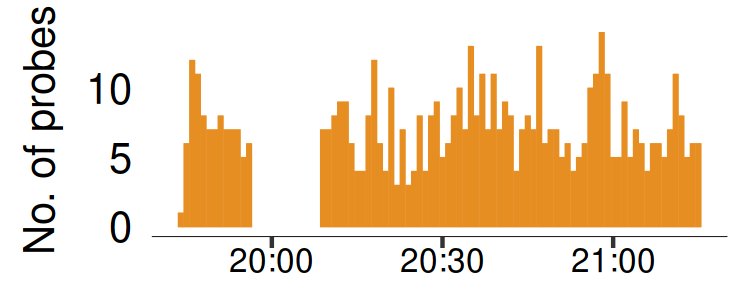
\includegraphics{images/home-total-count.png}
  \caption{Number of probe requests collected every minute on 15 October 2017}
  \label{figure:collection:home:total}
\end{marginfigure}

The first set of experiment was conducted with the laptop in the researcher's living room.
The primary aim of this experiment to collect an initial set of probe requests to understand the information in them.
The living room had 2 Wi-Fi enabled device - a motorola phone and an android tv 
The house had 2 more phones - iPhone and a Samsung phone.
Probe requests were collected on 15 Nov 2015 from 19:44 to 21:15 with a gap of 15 minutes in between.
We collected around 3000 probe requests at the rate of 38 requests per minute.

The first step was to look to convert these probe requests to number of devices by aggregating by the MAC addresses.
This results are shown in Figure \ref{figure:collection:home:total} which shows the number of unique MAC addresses detected every minute.
We see that aggregating by MAC addresses shows around 7 devices on average every minute around the sensor.
Though this might be true when considering noise from outside the room, it also reports around 211 unique MAC addresses overall these cannot be possibly generated by unique devices.
These unique addresses must have been caused by the randomisation process thus confirming that MAC addresses alone is not enough to convert the probe requests in to unique devices.

After this we looked at the resolved OUIs from the data.
There are 24 different vendors.
This is more than what we expected showing that these ones must be clearly coming from outside the room / house.
We need to find a way to look at the
We need to look at signal strength which can show how far the device is.
we look at the compression ration of MAC vs probes which shows the amount of randomisation.
Since we hashed the mac address there is no way of finding out. we need to keep the OUI part which is independent from vendor. Not all local OUIs are private.
Compex, Google and local addresses are randomising.
Samsung is tricky since we know that samsung phones don't randomise. we need to look into this more to see if it is randomisation.
nvidia, amazon, azurewav does not randomise.

%:read !tail -n +7 ./analysis/data-collection/vendor-tables.txt | head -n -3
\begin{table}
\footnotesize
\begin{center}
  \begin{tabular}{lrrrrrrrr}
  \toprule
  Vendor & Probe & MAC & Signal & Frame & Dura-& Tags & SSID & Sequence \\ 
  & request & address & strength & length &  tion &  &  & numbers \\ 
  \midrule
  AmazonTe &  101 &   1 & -80.53 &   4 &   4 &   5 &   3 & 101 \\ 
  Apple    &   77 &   7 & -86.29 &   4 &   4 &   9 &   4 &  77 \\ 
  ArrisGro &    7 &   1 & -91.71 &   1 &   1 &   1 &   1 &   7 \\ 
  Azurewav &  215 &   4 & -87.82 &   3 &   3 &  12 &  10 & 213 \\ 
  CompexPt &   75 &  28 & -88.17 &   3 &   3 &   5 &  29 &  74 \\ 
  CompexUs &    4 &   1 & -87.25 &   3 &   3 &   3 &   4 &   4 \\ 
  Dedicate &    2 &   1 & -92.50 &   1 &   1 &   1 &   1 &   2 \\ 
  Fn-LinkT &   64 &   1 & \textcolor{red}{-60.58} &   2 &   2 &   6 &   1 &  64 \\ 
  Google   & 1347 &  76 & \textcolor{red}{-69.14} &   4 &   5 &  41 &   6 & 1157 \\ 
  HuaweiTe &   11 &   3 & -87.91 &   3 &   3 &   3 &   1 &  11 \\ 
  IntelCor &   25 &   2 & -84.04 &   3 &   3 &   4 &   3 &  25 \\ 
  LenovoMo &    1 &   1 & -93.00 &   1 &   1 &   1 &   1 &   1 \\ 
  LgElectr &    1 &   1 & -90.00 &   1 &   1 &   1 &   1 &   1 \\ 
  Microsof &    3 &   1 & -90.00 &   1 &   1 &   1 &   2 &   3 \\ 
  Nvidia   &   65 &   1 & -82.91 &   2 &   2 &   4 &   2 &  65 \\ 
  OneplusT &    3 &   1 & -86.67 &   2 &   2 &   2 &   2 &   3 \\ 
  Pepwave  &    4 &   4 & -90.00 &   1 &   1 &   1 &   1 &   4 \\ 
  Sagemcom &    3 &   1 & -88.67 &   1 &   1 &   1 &   1 &   3 \\ 
  SamsungE &  655 &  27 & -83.81 &  26 &  26 &  54 &  23 & 621 \\ 
  SonyMobi &   56 &   2 & -78.66 &   2 &   2 &   2 &   1 &  56 \\ 
  TctMobil &    1 &   1 & -90.00 &   1 &   1 &   1 &   1 &   1 \\ 
  Tp-LinkT &   31 &   1 & -86.16 &   1 &   1 &   3 &   1 &  31 \\ 
  Wisol    &  143 &   3 & -71.91 &   4 &   5 &   6 &   3 & 142 \\ 
  XiaomiCo &    3 &   2 & -88.67 &   2 &   2 &   3 &   2 &   3 \\ 
  Unknown  &  110 &  40 & -88.86 &  19 &  18 &  21 &   5 &  90 \\ 
  \bottomrule
  \end{tabular}
\end{center}
\caption{Number of unique values present in each field captured from the probe requests for each Vendor OUI}
\label{table:collection:proberequest}
\end{table}

We then look at the average signal strength.
Only two of the vendors have averages less than 70 showing the only two devices that are in the room.
Rest of the devices are more than 80. Showing the exponential decay of the signal strength as we cross walls.
Signal strength can be a good indicator to isolate devices based on their distance from the sensor.
Figure shows the distribution of the signal strengths, we can clearly see inside and outside the room from the distribution.
We found that it is not enough.

We then look at all the other information we collected from the probe requests and see how they compare to the MAC address for aggregating.
We see length, duration provides provides better aggregation fields than MAC whent he addresses are randomised.
The logic behind this is that since the phones are essentially sending the same information over and over with just changed MAC addresses (which is of fixed length) same phones should be sending packets of same length.
We also see that duration of the transfer being a function of the length of the packet almost same as unique as the length.
We can say there is no additional information encoded within the duration more than the length of the packet.
Tags and SSIDs though looked promising, doesn't give us enough unique finger print for the device.
Tags don't have much uniqueness device-wise and SSID information is sparse.
This is because of most of the devices don't have this field 66\% of local OUIs , 50\% of Google and 38\% of samsung probes dont have any SSID information.

\begin{figure}
  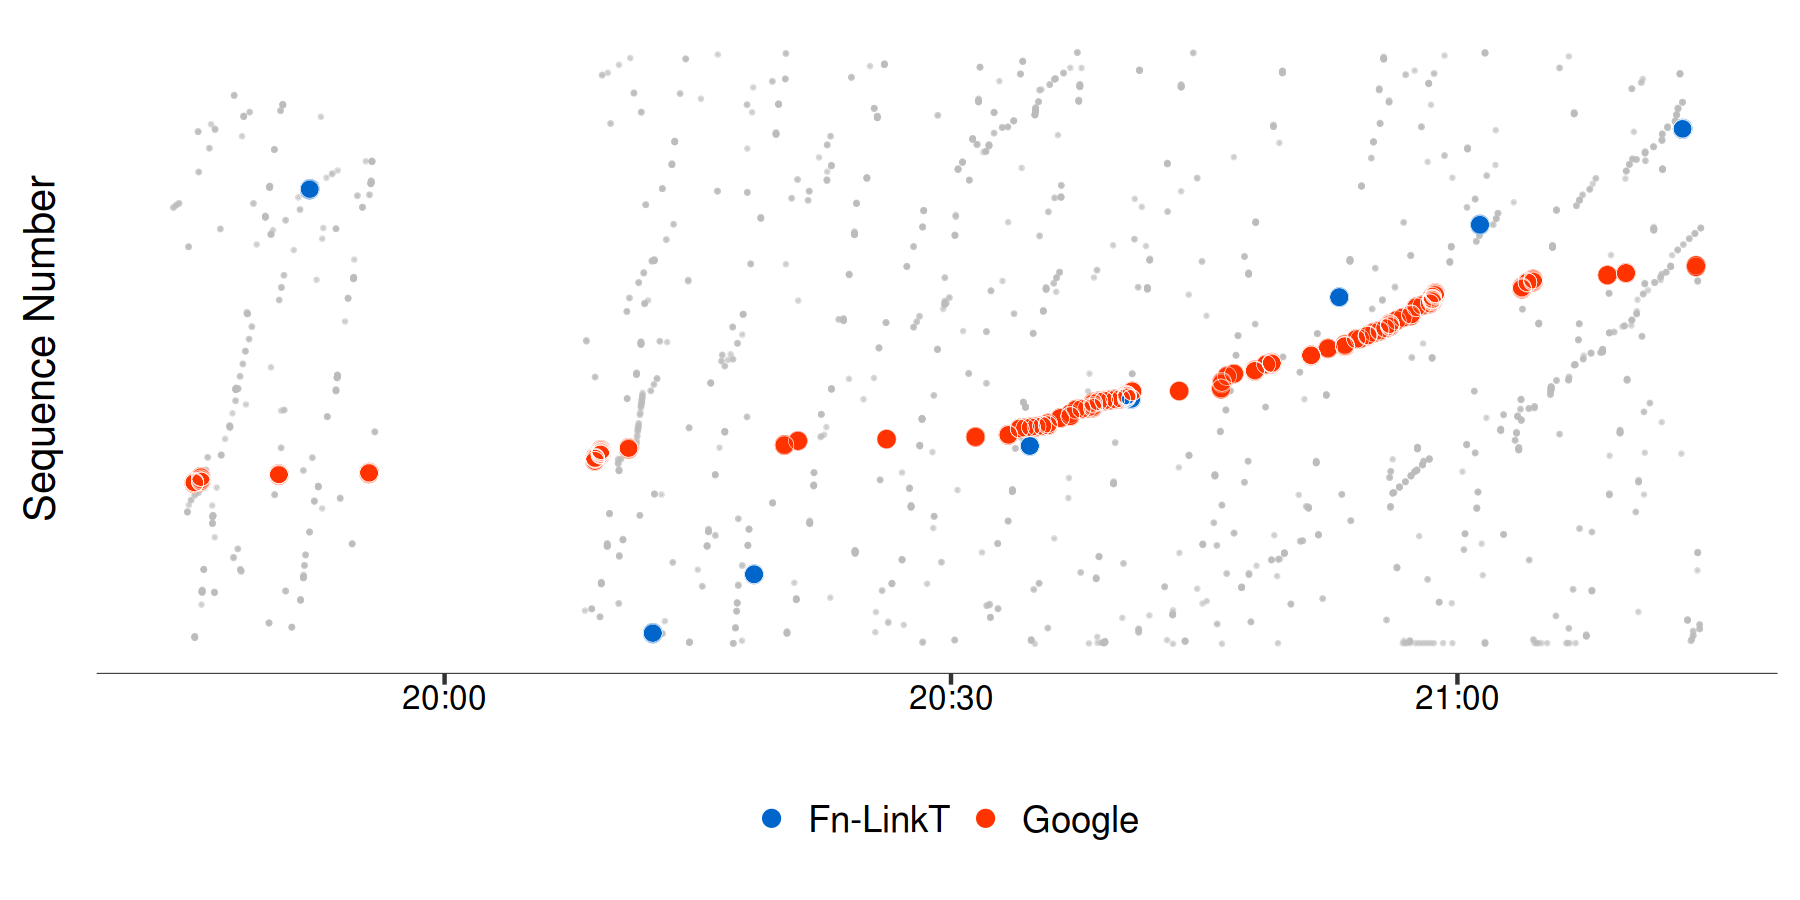
\includegraphics{images/home-sequence-time.png}
  \caption{Tree-map showing the volume of research conducted under each major themes and their sub-themes.}
  \label{figure:collection:home:sequence}
\end{figure}

Finally the sequence numbers are the most interesting part of the data collected. Though they don't uniquely identify the devices directly, along with timestamps they form visually discernible, unique patterns.
Figure \ref{figure:collection:home:sequence} we have isolated the two vendors and the probes with more than -70dBm and plotted their sequence numbers along with time. We can clearly see two devices which were present in the room. This shows the usefulness of the sequence number in estimating the actual devices around the sensors.
rotation of sequence numbers at 4096. This needs to be considered .
Figure \ref{figure:collection:home:samsung} shows a similar exploration of Samsung devices.
Though from the table \ref{table:collection:proberequest} it looked as if Samsung devices are randomising their MAC addresses, we can clearly that the diversity of MAC addresses are indeed unique devices which were far away from the sensor.
Though the results of this exploratory analysis has been positive the main challenge is to make sure these methods are feasible when dealing with more real-time, real world data.
We need to devise a more real world experiment to see frame lengths and signal strength work in a bigger data set for filtering out the noise. 

\begin{marginfigure}[-4cm]
  \forcerectofloat
  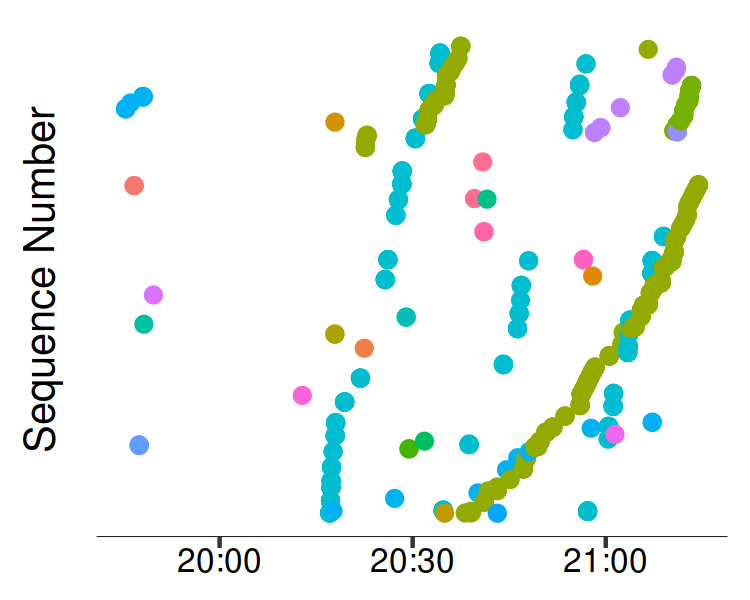
\includegraphics{images/home-samsung-google.png}
  \caption{Number of probe requests collected every minute on 15 October 2017}
  \label{figure:collection:home:samsung}
\end{marginfigure}
\marginnote{\textit{The colors show unique MAC addresses.} }

%------------------------------------------------------------------------------%
\subsection{University Hall}
%------------------------------------------------------------------------------%
This experiment was conducted to examine the previous results in a larger set of data in a more `real world' setting.
The specific goals are to validate the finding on signal strength corresponding to the distance from the sensor and to further examine the usefulness of the length parameter before collecting data on a busy retail setting.
Conducted in one of the main corridors - Southern cloisters of UCL with lot of pedestrian traffic.
There were also seating areas across the corridor where students work with their computers.
The area is also used heavily for lunch for large contingent of visitors.
Collected around 14750 probe requests collected and 652 users were counted walking around the sensors manually.

\begin{marginfigure}
  \forceversofloat
  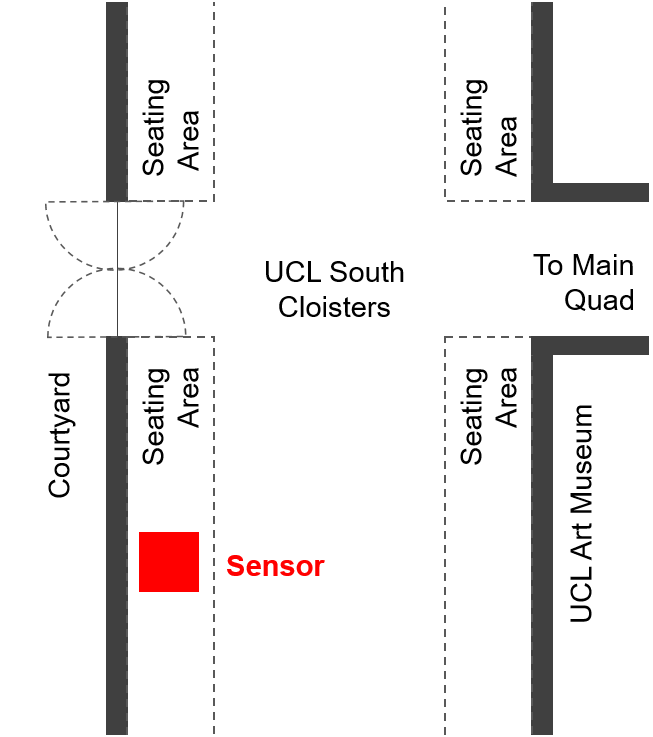
\includegraphics[trim={5 5 5 5},clip]{images/south-cloisters.png}
  \caption{Number of probe requests collected every minute on 15 October 2017}
  \label{figure:collection:ucl:config}
\end{marginfigure}
\marginnote{\textit{* Not to scale.} }

Major conclusion is that confirmation that Signal strength is still useful.
Length information is not that useful in certain standardised manufacturers.
At larger scales the manual counting is not possible without errors need to make a better alternative.

%------------------------------------------------------------------------------%
\subsection{Oxford Street}
%------------------------------------------------------------------------------%

Aim is to validate the filtering and clustering methodology against the scale and complexity of data collected in an open public area such as a retail high street.
We also aimed to find the algorithm which was best suited for the classification of signal strengths as 'low' and 'high' in order to filter out the background noise.
The data was collected at Oxford Street, London on 20 December 2017 from 12:30 to 13:00 hrs, Wi-Fi probe requests were collected using the sensor described in Section and pedestrian footfall was manually recorded using node-js based software, included in appendix.
Being located at one of the busiest retail locations in the United Kingdom, the Wi-Fi sensor captured approximately 60,000 probe requests during the half hour period; 3,722 people were manually recorded walking on the pavement during that time.
The surveyor positioned himself at the front of a store while carrying the sensor in a backpack and counted people walking by the store on the pavement (3m wide approximately) using a mobile phone.
The sensor was kept as close to the store window as possible, and the manual count was done as a cordon count in front of the store.

The analysis and use of this dataset is 

%------------------------------------------------------------------------------%
\subsection{Outputs from the experiments}
%------------------------------------------------------------------------------%

Probe requests are source of easy to collect rich information.
We identified list of useful information we can get from them.
We collected data in three phases starting from small isolated study, more footfall and real world retail location.
The first experiment showed that MAC address is not enough. Local mac addressed can be publicly registered as well.
Signal strength is crucial.
The broader UCL experiment in UCL corridor showed that though length information looked useful, it fails with apple devices since they are very similar to each other and lack any information elements. 
This gave us a good idea of what to collect in a field study. 
We collected data at Oxford street as a dataset for to be used as a starting point for any methodology we develop further.

%==============================================================================%
